\section{Bayesian Network}
\label{sec:design:bayesian-network}

Determining the correct action to trigger based on the contextual information is done using a Bayesian network. The network is illustrated in \cref{fig:design:bayesian-network:overview}. We consider there to be the following three levels in the network.

\begin{itemize}
\item The uppermost level containing the ``Gesture'', ``Room'', ``TV\_IsOn'' and ``MusicCentre\_IsPlaying'' nodes provides contextual information.
\item The middle level observes, \ie~is children of, the uppermost level to provide probabilities for each action in the system based on a subset of the information observed in the uppermost level.
\item The bottom level observes all nodes in the middle level to provide probabilities for the actions in the system. Based on these probabilities the correct action to perform is determined.
\end{itemize}

The benefit of this structure is, that contextual information such as the performed gesture and the users position is always translated to probabilities for actions and these probabilities are independent of other contextual information that we may observe. When the contextual information is modelled as probabilities for actions, it becomes trivial to combine all the contextual information to choose the right action to perform.

The probability tables and conditional probability tables shown in \cref{tbl:design:bayesian-network:pt-gesture-room,tbl:design:bayesian-network:pt-tv-ison-musiccentre-isplaying,tbl:design:bayesian-network:cpt-gesture-action,tbl:design:bayesian-network:cpt-room-action,tbl:design:bayesian-network:cpt-system-state-action,tbl:design:bayesian-network:cpt-action} only show selected states. In reality, the tables include states for all gestures, rooms and actions in the system but some have been left out for readability purposes.

\begin{figure}[h!]
\centering
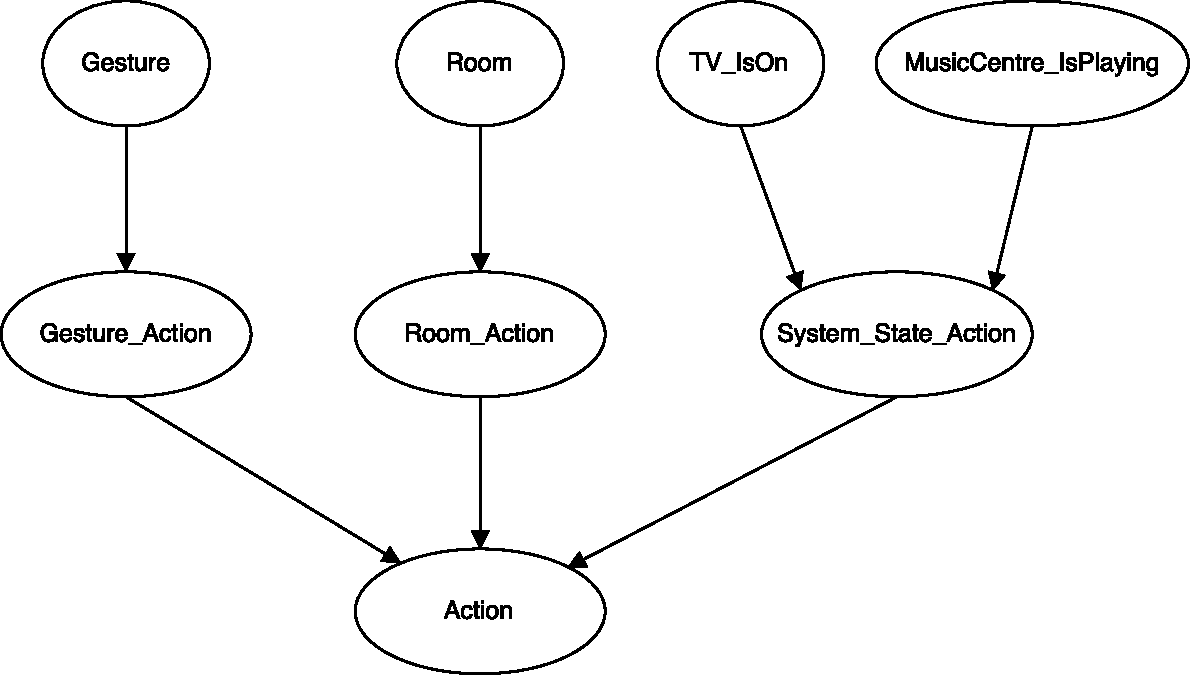
\includegraphics[width=0.75\textwidth]{images/bayesian-network}
\caption{The Bayesian network used for determining the appropriate action to trigger based on the gesture performed by the user, the position of the user and the state of the system.}
\label{fig:design:bayesian-network:overview}
\end{figure}

\Cref{tbl:design:bayesian-network:pt-gesture-room} shows an excerpt of the probability table for the gesture node. The node contains probabilities for all gestures in the system. The probability is the same for all gestures in the system. This is because the user is equally likely to have performed the gestures when we have not observed anything else. Based on the likelihoods of each gesture supplied by the gesture recognizer, we can add soft evidence to the Gesture node. The evidence is assigned as described in \cref{sec:design:bayesian-network:gesture-node-evidence}.

When using a Bayesian network, we assign evidence to the states of a node. If a node, $X$, in a bayesian network has states $x_1$, $x_2$ and $x_3$ then an evidence function $\epsilon_X = (1, 0, 0)$ indicates that $X = x_1$, \ie~node $X$ is in state $x_1$ with certainty. If $\epsilon_X = (1, 2, 0)$ then we are sure that $X$ is not in state $x_3$ and $X = x_2$ is twice as likely as $X = x_1$ \cite[pp. 23-24]{kjaerulff2008bayesian}. The probabilities for a column in a conditional probability table should have a sum of 1. That is for a node $X$, $P(x_1) + P(x_2) + ... + P(X_n) = 1$ where $n$ is the number of states in $X$.

As per Kjærulff \etal\cite[pp. 23-24]{kjaerulff2008bayesian} we distinquish between \emph{hard evidence} and \emph{soft evidence}. If an evidence function assigns a probability of zero to all but one state in a node, then there is \emph{hard evidence} on that one state. If an evidence function assigns evidence to multiple states, there is said to be \emph{soft evidence} on the states.

\begin{table}[h!]
\centering
\caption{Excerpt of the probability tables for the Gesture and Room nodes.}
\label{tbl:design:bayesian-network:pt-gesture-room}
\begin{tabular}{cc}
\begin{tabular}{c}
\textbf{Gesture}   \\
\begin{tabular}{ccc}
Z   & Half circle & Horizontal line \\ \hline
$\frac{1}{3}$ & $\frac{1}{3}$         & $\frac{1}{3}$
\end{tabular}
\end{tabular}
&
\begin{tabular}{c}
\textbf{Room}   \\
\begin{tabular}{ccc}
Bedroom   & Living room \\ \hline
0.5 & 0.5
\end{tabular}
\end{tabular}
\end{tabular}
\end{table}

\begin{table}[h!]
\centering
\caption{Probability tables for the TV\_IsOn and MusicCentre\_IsPlaying nodes.}
\label{tbl:design:bayesian-network:pt-tv-ison-musiccentre-isplaying}
\begin{tabular}{cc}
\begin{tabular}{c}
\textbf{TV\_IsOn}   \\
\begin{tabular}{cc}
Yes   & No \\ \hline
0.5 & 0.5
\end{tabular}
\end{tabular}
&
\begin{tabular}{c}
\textbf{MusicCentre\_IsPlaying}   \\
\begin{tabular}{cc}
Yes   & No \\ \hline
0.5 & 0.5
\end{tabular}
\end{tabular}
\end{tabular}
\end{table}

The Gesture, Room, TV\_IsOn and MusicCentre\_IsPlaying nodes constitute the uppermost level in the network. The middle level is constituted by the Gesture\_Action, Room\_Action and System\_State\_Action nodes.

The nodes on the middle level observes nodes in the uppermost level and based on the observed information, compute probabilities for the all actions in the system. Without any evidence on a state, the probabilities of the states in nodes in the middle level is determined by gesture configurations.

Consider the probabilities of the Gesture\_Action node as shown in \cref{tbl:design:bayesian-network:cpt-gesture-action}. In the scenario presented in \cref{sec:analysis:scenarios} we presented a configuration of the system. \Cref{tbl:design:bayesian-network:cpt-gesture-action} shows an excerpt of the configuration in which the user has configured the Z gesture to turn Lamp 3 and Lamp 8 on and off. The Half Circle gesture skips to the next track on the music centre and changes to the next channel on the television. The Horizontal Line gesture skips to the previous track on the music centre and changes to the previous channel on the television. The valid actions for each gesture have the same probability.

As the Gesture\_Action node observes the Gesture node, the probabilities of each action are changed when evidence is added to the states of the Gesture node.

\begin{table}[h!]
\centering
\caption{Excerpt of the conditional probability table for the Gesture\_Action node.}
\label{tbl:design:bayesian-network:cpt-gesture-action}
\begin{tabular}{c}
\textbf{Gesture\_Action}   \\
\begin{tabular}{l|ccc}
                             & Z   & Half circle & Horizontal line \\ \hline
Lamp 3: on/off               & 0.5 & 0             & 0                \\
Lamp 8: on/off               & 0.5 & 0             & 0                \\
Music centre: next track     & 0   & 0.5             & 0                \\
Music centre: previous track & 0   & 0             & 0.5              \\
Television: next channel     & 0   & 0.5             & 0                \\
Television: previous channel & 0   & 0             & 0.5              
\end{tabular}
\end{tabular}
\end{table}

The principle oof the Room\_Action and System\_State\_Action nodes are the same as the Gesture\_Action node. Each state of the nodes correspond to an action in the system. The probabilities of the nodes change when evidence is added to the Room, MusicCentre\_IsPlaying and TV\_IsOn nodes.

The evidence added to the states of the Room node, is likely to be soft evidence as we adjust the probability of the user being in a room over time as he walks around as described in \cref{sec:design:bayesian-network:room-node-evidence}. The evidence of the MusicCentre\_IsPlaying and TV\_IsOn nodes are hard evidence as we can observe this with certainity from the state of items in openHAB.

\begin{table}[h!]
\centering
\caption{Excerpt of the conditional probability table for the Room\_Action node.}
\label{tbl:design:bayesian-network:cpt-room-action}
\begin{tabular}{c}
\textbf{Room\_Action}   \\
\begin{tabular}{l|cc}
                             & Bedroom & Living room \\ \hline
Lamp 3: on/off               & 0 & $\frac{1}{3}$ \\
Lamp 8: on/off               & $\frac{1}{3}$ & 0 \\
Music centre: next track     & 0   & $\frac{1}{3}$ \\
Music centre: previous track & 0    & $\frac{1}{3}$ \\
Television: next channel     & $\frac{1}{3}$   & 0  \\
Television: previous channel & $\frac{1}{3}$   & 0  \\
\end{tabular}
\end{tabular}
\end{table}

\begin{table}[h!]
\centering
\caption{Excerpt of the conditional probability table for the System\_State\_Action node.}
\label{tbl:design:bayesian-network:cpt-system-state-action}
\begin{tabular}{c}
\textbf{System\_State\_Action}   \\
\begin{tabular}{l|cc}
MusicCentre\_IsPlaying       & Yes & No \\
TV\_IsOn                     & 
\begin{tabularx}{2cm}{YY} Yes & No \end{tabularx}
&
\begin{tabularx}{2cm}{YY} Yes & No \end{tabularx}
\\ \hline
Lamp 3: on/off               & 
\begin{tabularx}{2cm}{YY} $\frac{1}{6}$ & 0.25 \end{tabularx}
&
\begin{tabularx}{2cm}{YY} 0.25 & 0.5 \end{tabularx}
\\
Lamp 8: on/off               & 
\begin{tabularx}{2cm}{YY} $\frac{1}{6}$ & 0.25 \end{tabularx}
&
\begin{tabularx}{2cm}{YY} 0.25 & 0.5 \end{tabularx}
\\
Music centre: next track               & 
\begin{tabularx}{2cm}{YY} $\frac{1}{6}$ & 0.25 \end{tabularx}
&
\begin{tabularx}{2cm}{YY} 0 & 0 \end{tabularx}
\\
Music centre: previous track               & 
\begin{tabularx}{2cm}{YY} $\frac{1}{6}$ & 0.25 \end{tabularx}
&
\begin{tabularx}{2cm}{YY} 0 & 0 \end{tabularx}
\\
Television: next channel               & 
\begin{tabularx}{2cm}{YY} $\frac{1}{6}$ & 0 \end{tabularx}
&
\begin{tabularx}{2cm}{YY} 0.25 & 0 \end{tabularx}
\\
Television: previous channel               & 
\begin{tabularx}{2cm}{YY} $\frac{1}{6}$ & 0 \end{tabularx}
&
\begin{tabularx}{2cm}{YY} 0.25 & 0 \end{tabularx}
\end{tabular}
\end{tabular}
\end{table}

Based on the information observed from the Gesture\_Action, Room\_Action and System\_State\_Action nodes, the Action node calculates probabilities of each action in the system. The probabilities of the node are used to determine which action to trigger.

\Cref{tbl:design:bayesian-network:cpt-action} shows a very small excerpt of the conditional probability table of the Action node. For readability purposes the table only contains two states, A and B. We assume A and B are actions in the system. For example, $\text{A} = \text{``Lamp 3: on/off''}$ and $\text{B} = \text{``Music centre: next track''}$.

When System\_State\_Action = $A_1$, Room\_Action = $A_1$ and Gesture\_Action = $A_1$ there is hard evidence that action A should be triggered. The same applies for action $A_2$ when all three nodes are in state $A_2$. If only two two nodes are in state $A_1$, then the probability of $P(Action=A_1) = \frac{2}{3}$ and as a result $P(Action=A_2) = \frac{1}{3}$ and vice versa.

\begin{table}[h!]
\centering
\caption{Excerpt of the conditional probability table for the Action node in the Bayesian network presented in \cref{fig:design:bayesian-network:overview}.}
\label{tbl:design:bayesian-network:cpt-action}
\begin{tabular}{c}
\textbf{Action} \\
\begin{tabular}{l|c}
System\_State\_Action & \begin{tabularx}{11cm}{Y|Y} $A_1$ & $A_2$ \end{tabularx} \\ \hline
Room\_Action          & \begin{tabularx}{11cm}{Y|Y|Y|Y} $A_1$ & $A_2$ & $A_1$ & $A_2$ \end{tabularx} \\ \hline
Gesture\_Action       & \begin{tabularx}{11cm}{YY|YY|YY|YY} $A_1$ & $A_2$ & $A_1$ & $A_2$ & $A_1$ & $A_2$ & $A_1$ & $A_2$ \end{tabularx} \\ \hline
A                     & \begin{tabularx}{11cm}{YY|YY|YY|YY} 1 & $\frac{2}{3}$ & $\frac{2}{3}$ & $\frac{1}{3}$ & $\frac{2}{3}$ & $\frac{1}{3}$ & $\frac{1}{3}$ & 0 \end{tabularx} \\ 
B                     & \begin{tabularx}{11cm}{YY|YY|YY|YY} 0 & $\frac{1}{3}$ & $\frac{1}{3}$ & $\frac{2}{3}$ & $\frac{1}{3}$ & $\frac{2}{3}$ & $\frac{2}{3}$ & 1 \end{tabularx}
\end{tabular}
\end{tabular}
\end{table}

\subsection{Evidence in Gesture Node}
\label{sec:design:bayesian-network:pgesture-node-evidence}

The following section describes how the evidence assigned to the states in the Gesture node of the Bayesian network is determined. In order to determine the evidence, we introduce the \emph{gesture context provider}.

The gesture context provider determines the actions that make sense to trigger based on the motion performed by the user. When the user performs a motion, the gesture recognizer scores the trained gestures as explained in \cref{sec:design:gesture-recognition}. When the gestures are scored, they are passed to the context provider which calculates the probabilities of each action associated with the gesture. The calculation of probabilities is similar to the calculation of probabilities for the position context provider presented in \cref{sec:design:bayesian-network:room-node-evidence}.

When calculating the probabilities, all actions associated with each gesture is retrieved, the scores are normalized and distributed among the actions.

For example, if gestures $G_1$ and $G_2$ are recognized with $G_1$ having a score of 47 and $G_2$ having a score of 93, the total score is $47 + 93 = 140$. Assume that $G_1$ is associated with actions 1 and 2 and $G_2$ is associated with action 3.

The lower the score is, the better. Therefore the probability of gesture $G_1$ being recognized is considered to be the following.

\begin{equation*}
(1 - \frac{47}{140}) \cdot 100 = 66.43
\end{equation*}

The probability of gesture $G_2$ is considered to be the following.

\begin{equation*}
(1 - \frac{93}{140}) \cdot 100 = 33.57
\end{equation*}

The normalized probabilities are used as soft evidence of the states in the Gesture node.

%%% Local Variables:
%%% mode: latex
%%% TeX-master: "../../master"
%%% End:

\subsection{Evidence in Room Node}
\label{sec:design:bayesian-network:room-node-evidence}

The following section describes how the evidence assigned to states in the Room node of the Bayesian network is determined. In order to determine the evidence, we introduce the \emph{position context provider}.

The position context provider is responsible for determining which actions make sense to trigger given the users current position. For each action it provides the likelihood of those actions being the intended ones. The likelihoods are the evidence assigned to the states in the Room node.

The context provider determines the position of the user using BLE. One or more Estimote beacons are installed in rooms that should be tracked. The beacons broadcast using the Eddystone protocol as described in \Cref{sec:design:ble-positioning}. The wearable continuously scans for nearby beacons using the Estimote SDK.

The Estimote beacons delivers a set of discovered beacons several times each second. Each time beacons are discovered, the provider chooses the beacon with the highest RSSI. We assume that the higher the RSSI is, the closer the user is to the beacon as the RSSI is an indicator of the signal strength between the two Bluetooth devices.

In order to account for sporadic and false measurements indicating that the user is in the wrong room, we store a reference to the room in which the beacon with the highest RSSI is placed. Each reference lives in the queue for 30 seconds. We keep each reference for 30 seconds, because Estimote estimates that a region exit in their SDK usually takes up to 30 seconds and therefore we make the same assumption~\cite{estimote:beacon-monitoring}. Whenever the context provider is asked to provide its context, we calculate the occurrence of each beacon in percentage. For example, consider the following set where $R_1$, $R_2$ and $R_3$ are different rooms.

\begin{equation*}
  \{ R_1, R_1, R_2, R_2, R_1, R_1, R_1, R_2, R_3, R_1, R_1, R_1 \}
\end{equation*}

There are a total of twelve items in the queue. $R_1$ occurs eight times, $R_2$ occurs three times and $R_3$ occurs one time. Therefore we assign a 66.67\% probability that the user is in $R_1$, a 25\% probability that the user is in $R_2$ and a roughly 8.33\% probability that the user is in $R_3$. The normalized probabilities are used as soft evidence of the states in the Room node.

%%% Local Variables:
%%% mode: latex
%%% TeX-master: "../../master"
%%% End:

\subsection{Evidence in System State Nodes}
\label{sec:design:bayesian-network:system-state-nodes-evidence}

In \cref{fig:design:bayesian-network:overview} we suggested two nodes that supply information about the system state. The TV\_IsOn supplies information about whether not the television is on and the MusicCentre\_IsPlaying node supplies information on whether or not the music centre is playing music. Naturally these are examples of nodes that can describe the state of the system. Other examples can include if a lamp is on or not, a door is locked or unlocked or who is home.

In \cref{fig:design:bayesian-network:overview} the TV\_IsOn and MusicCentre\_IsPlaying nodes are parents of the System\_State\_Action node. An alternative model for the system state is illustrated in \cref{fig:design:bayesian-network:system-state-nodes-evidence:alternative-network}. 

\begin{figure}[h!]
\centering
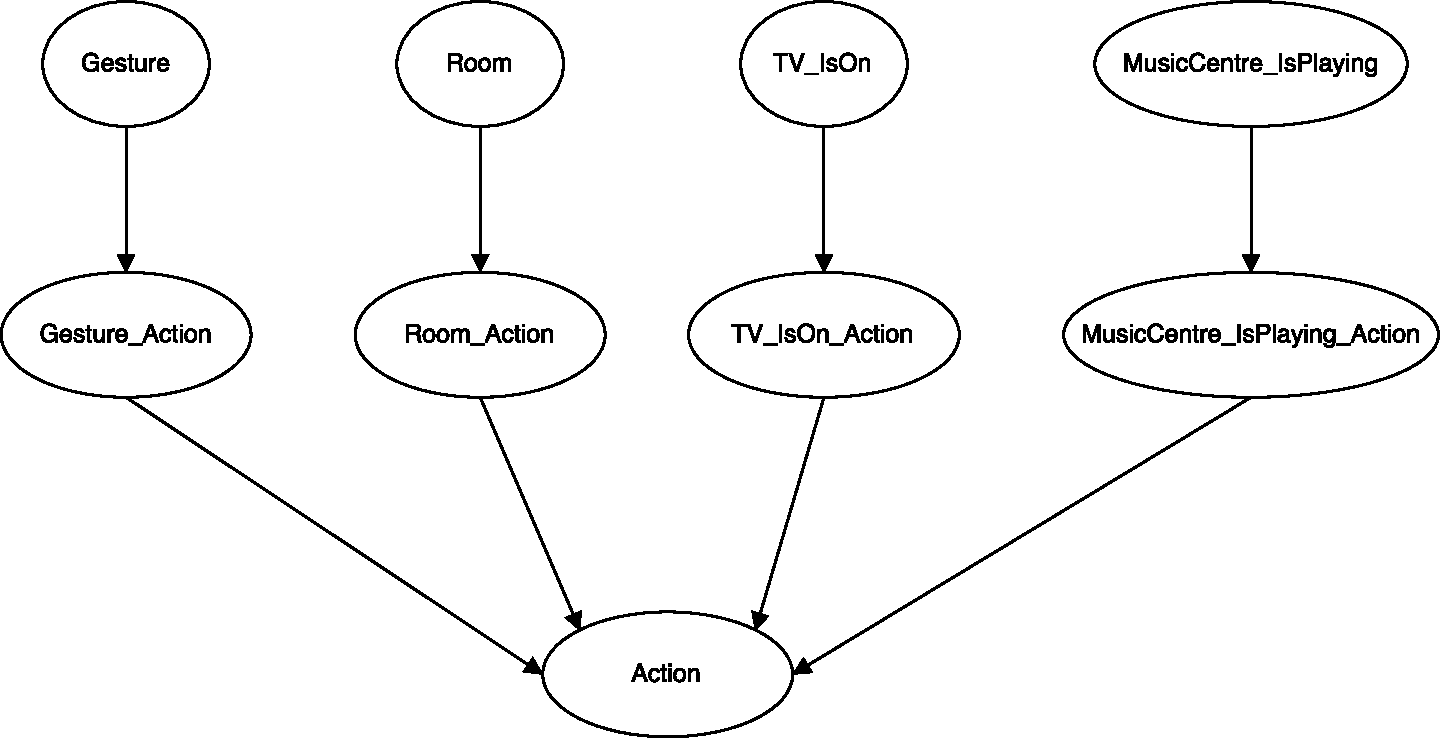
\includegraphics[width=0.75\textwidth]{images/bayesian-network-split-system-state}
\caption{Alternative apporach for modeling the system state in the Bayesian network.}
\label{fig:design:bayesian-network:system-state-nodes-evidence:alternative-network}
\end{figure}

The System\_State action node have been replaced by the TV\_IsOn\_Action and MusicCentre\_IsPlaying\_Action nodes. Each observes a specific part of the system state. The conditional probability tables for the nodes are shown in \cref{tbl:design:bayesian-network:system-state-nodes-evidence:alternative-system-state}.

Consider the table for TV\_IsOn\_Action with a subset of the actions presented in the scenario. As the node knows nothing about the state of the television, it must have equal probabilities for the two states when the television is on. However, if the television is off the node has zero probability of changing the channel on the television. The same principle applies for the MusicCentre\_IsPlaying\_Action node.

\begin{table}[h!]
\centering
\caption{Probability tables for the TV\_IsOn\_Action and MusicCentre\_IsPlaying\_Action nodes in the alternative Bayesian network illustrated in \cref{fig:design:bayesian-network:system-state-nodes-evidence:alternative-network}.}
\label{tbl:design:bayesian-network:system-state-nodes-evidence:alternative-system-state}
\begin{tabular}{cc}
\begin{tabular}{c}
\textbf{TV\_IsOn\_Action}   \\
\begin{tabular}{l|cc}
~ & Yes   & No \\ \hline
Music centre: next track & 0.5 & 1 \\
Television: next channel & 0.5 & 0
\end{tabular}
\end{tabular}
&
\begin{tabular}{c}
\textbf{MusicCentre\_IsPlaying\_Action}   \\
\begin{tabular}{l|cc}
~ & Yes   & No \\ \hline
Music centre: next track & 0.5 & 0 \\
Television: next channel & 0.5 & 1
\end{tabular}
\end{tabular}
\end{tabular}
\end{table}

The influence of the system state is illustrated in figures \ref{fig:design:bayesian-network:evidence-system-state-nodes:system-state-1} and \ref{fig:design:bayesian-network:evidence-system-state-nodes:system-state-2}. For readability purposes the illustrated networks only contains a subset of the scenarios presented in \cref{sec:analysis:scenarios}. In the first figure the system state has little influence. The television is on and the music is playing but because the user is in the living room, the action is triggered on the music centre. In the second figure, an action is triggered in the bedroom even though there is evidence that the user is in the living room. The ``Music centre: next track'' is not triggered as the music centre is not playing. However, the gesture has a meaning in the bedroom from which there is little evidence that the user is in. Therefore the action is triggered in the bedroom. Had there been hard evidence that the user is in the living room, the actions would have had the same probability and the system would ask the user which of the two actions he desired to trigger.

\begin{figure}[h!]
\centering
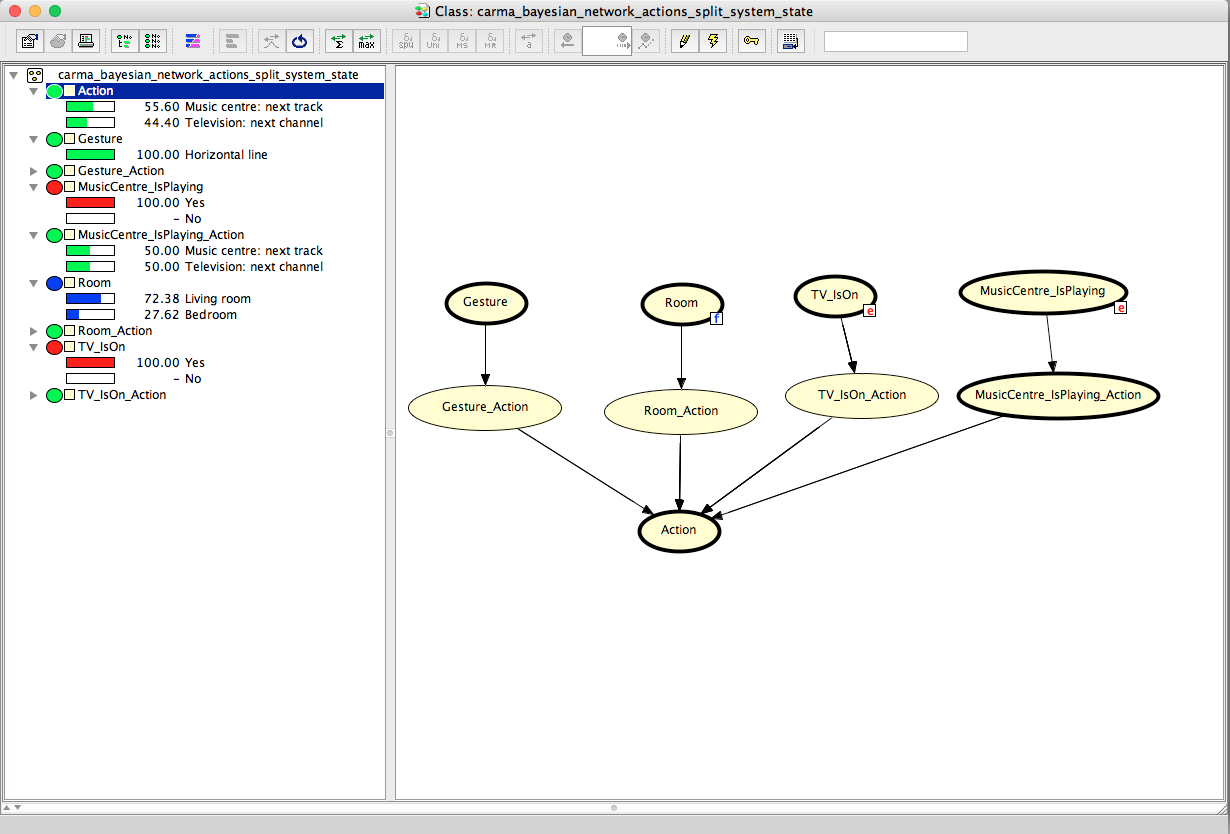
\includegraphics[width=\textwidth]{images/bayesian-split-system-state-1}
\caption{Example Bayesian network with origin in the scenario presented in \cref{sec:analysis:scenarios}. The network has a single gesture, a probability of 72.38\% that the user is in the living room and 27.62\% that he is in the bedroom. The user is in the living room. The television is turned on and the music is playing. Because the user is in the living room, the music is changed when the Horizontal Line gesture is performed. Green bars indicate probabilities, red bars indicate hard evidence and blue bars indicate soft evidence.}
\label{fig:design:bayesian-network:evidence-system-state-nodes:system-state-1}
\end{figure}

\begin{figure}[h!]
\centering
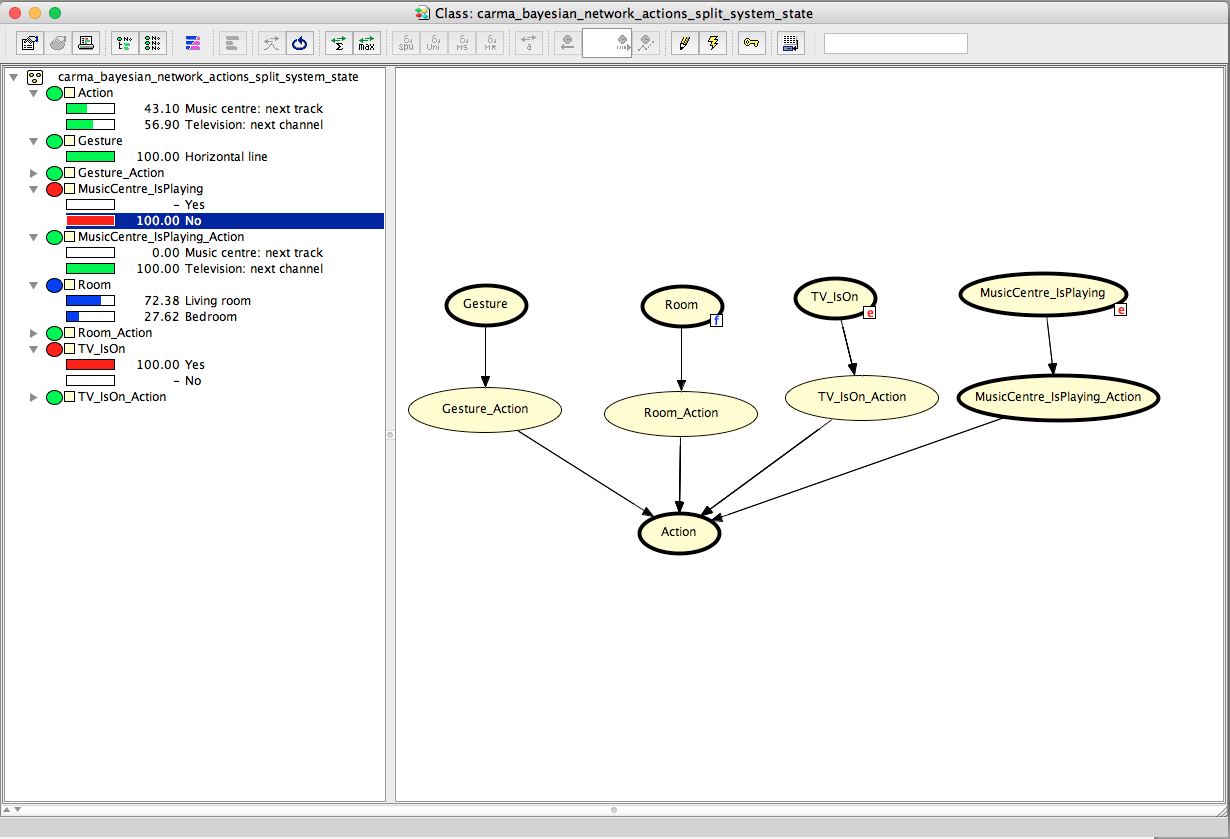
\includegraphics[width=\textwidth]{images/bayesian-split-system-state-2}
\caption{Example Bayesian network with origin in the scenario presented in \cref{sec:analysis:scenarios}. The network has a single gesture, a probability of 72.38\% that the user is in the living room and 27.62\% that he is in the bedroom. While the user is in the living room, the action in the bedroom is performed when the user triggers a gesture because the action in the living room is not valid according to the system state. Green bars indicate probabilities, red bars indicate hard evidence and blue bars indicate soft evidence.}
\label{fig:design:bayesian-network:evidence-system-state-nodes:system-state-2}
\end{figure}

As illustrated in figures \ref{fig:design:bayesian-network:evidence-system-state-nodes:system-state-1} and \ref{fig:design:bayesian-network:evidence-system-state-nodes:system-state-2} evidence on the system state is hard. The system state can be obtained from the items in openHAB and assuming that we can trust the data delivered by openHAB, we can be sure of the system state.

%%% Local Variables:
%%% mode: latex
%%% TeX-master: "../../master"
%%% End:


%%% Local Variables:
%%% mode: latex
%%% TeX-master: "../../master"
%%% End:
